\section{Basic Tutorials 2}

%%%%%%%%%%%%%
\subsection{Filters}

%% Break
\begin{frame}{Basic Tutorial 2}
\fontsize{36pt}{36pt}\selectfont
\center
\begin{center}
Basic Tutorial 2
\end{center}
\end{frame}

\begin{frame}[fragile]
\frametitle{Filter Anatomy}
\begin{center}
  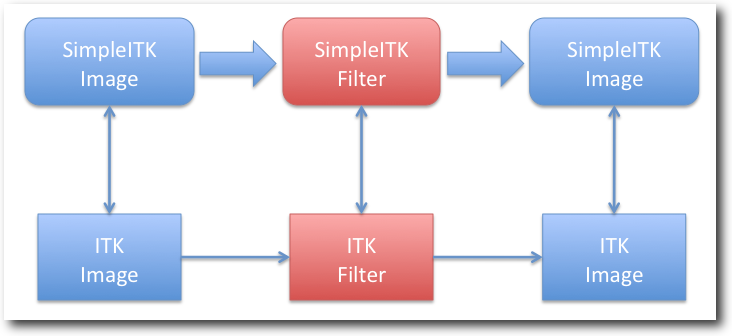
\includegraphics[width=.8\textwidth]{Images/FilterOverview_shadow}
\end{center}
\begin{itemize}
  \item SimpleITK filters create ITK filters
  \item Templated based on input type
  \item Output type is usually the same as input type
  \item Instantiated for many possible image types
\end{itemize}
\end{frame}

\begin{frame}[fragile]
\frametitle{Image and Filter Types}
\begin{columns}
  \begin{column}{0.5\textwidth}
    \begin{itemize}
      \item Dimensions
      \begin{itemize}
        \item 2 dimensional
        \item 3 dimensional
      \end{itemize}
      \item Scalar types
      \begin{itemize}
        \item $int8\_t$
        \item $uint8\_t$
        \item $int16\_t$
        \item $uint16\_t$
        \item $int32\_t$
        \item $uint32\_t$
        \item $float$
        \item $double$
        \item $std::complex< float >$
        \item $std::complex< double >$
      \end{itemize}
    \end{itemize}
  \end{column}

  \begin{column}{0.5\textwidth}
     \begin{itemize}
       \item Vector Types
       \begin{itemize}
         \item $int8\_t$
         \item $uint8\_t$
         \item $int16\_t$
         \item $uint16\_t$
         \item $float$
         \item $double$
       \end{itemize}
       \item Label Types
       \begin{itemize}
         \item $uint8\_t$
         \item $uint16\_t$
         \item $uint32\_t$
       \end{itemize}
    \end{itemize}
  \end{column}
\end{columns}
\end{frame}

\begin{frame}[fragile]
\frametitle{Filter Anatomy}
\begin{center}
  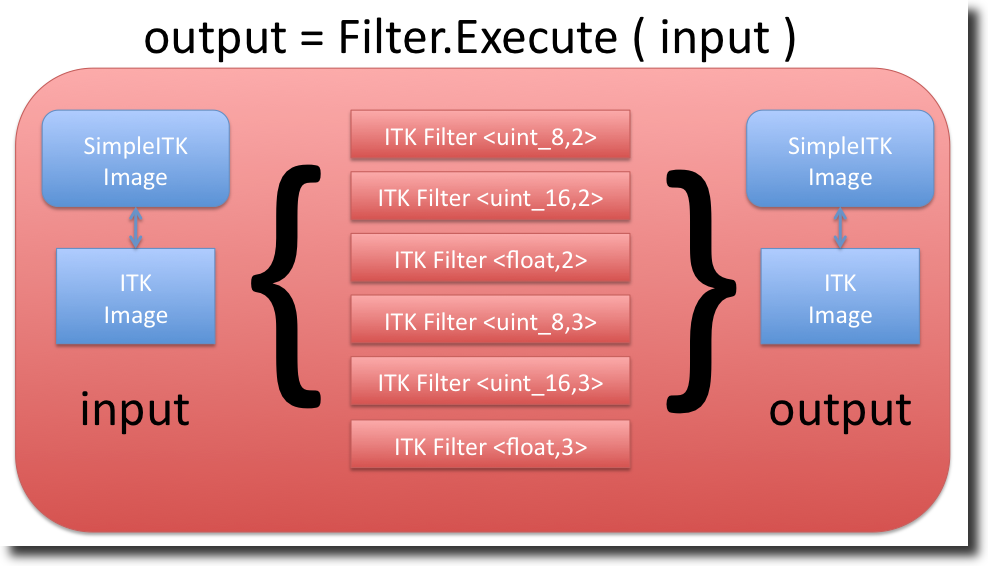
\includegraphics[width=.8\textwidth]{Images/FilterInternals_shadow}
\end{center}
\begin{itemize}
  \item Filter interrogates $input$
  \item Instantiates proper ITK filter
  \item Executes ITK filter
  \item Constructs $output$ from ITK image
\end{itemize}
\end{frame}

\subsection{Code Philosophy}
\begin{frame}{Code Philosophy}
\fontsize{36pt}{36pt}\selectfont
\center
\begin{center}
Code Philosophy
\end{center}
\end{frame}

\begin{frame}[fragile]
\frametitle{Filter Class Overview (C++)}
\lstcpp
\begin{lstlisting}
class SmoothingRecursiveGaussianImageFilter : (* \label{Declaration} *)
    public ImageFilter {
  typedef SmoothingRecursiveGaussianImageFilter Self; (* \label{Self} *)

  /** Default Constructor that takes no arguments
      and initializes default parameters */
  SmoothingRecursiveGaussianImageFilter(); (* \label{Constructor} *)

\end{lstlisting}
\begin{itemize}
  \item In line \ref{Declaration}, we declare a subclass of ImageFilter
  \item Line \ref{Self} creates a special typedef for use later
  \item The default constructor is line \ref{Constructor} (never any parameters)
\end{itemize}
\end{frame}


\begin{frame}[fragile]
\frametitle{Filter Class Overview (C++) Continued}
\lstcpp
\begin{lstlisting}
  /** Define the pixels types supported by this filter */
  typedef BasicPixelIDTypeList  PixelIDTypeList; (* \label{PixelIDTypeList} *)

\end{lstlisting}
\begin{itemize}
  \item Notice $PixelIDTypeList$ in line \ref{PixelIDTypeList}
  \item Used to instantiate ITK filters
  \item Determines valid input image types
  \item $BasicPixelIDTypeList$ expands to:
  \begin{itemize}
    \item $int8\_t$, $uint8\_t$
    \item $int16\_t$, $uint16\_t$
    \item $int32\_t$, $uint32\_t$
    \item $float$, $double$
  \end{itemize}
\end{itemize}
\end{frame}


\begin{frame}[fragile]
\frametitle{Filter Class Overview (C++) Continued}
\lstcpp
\begin{lstlisting}
  Self& SetSigma ( double t ) { ... return *this; }
  double GetSigma() { return this->m_Sigma; }

  Self& SetNormalizeAcrossScale ( bool t ) { ... }
  Self& NormalizeAcrossScaleOn() { ... }
  Self& NormalizeAcrossScaleOff() { ... }

  bool GetNormalizeAcrossScale() { ... }
\end{lstlisting}
\begin{itemize}
  \item Get/Set parameters
  \item Set methods always return $Self\&$ (more later)
  \item Generally, a direct mapping to ITK
  \item Boolean parameters generate $On$ and $Off$ methods
\end{itemize}
\end{frame}


\begin{frame}[fragile]
\frametitle{Filter Class Overview (C++) Continued}
\lstcpp
\begin{lstlisting}
  /** Name of this class */
  std::string GetName() const { ... }

  /** Print ourselves out */
  std::string ToString() const;
\end{lstlisting}
\begin{itemize}
  \item Return the name and description of the filter
\end{itemize}
\end{frame}


\begin{frame}[fragile]
\frametitle{Filter Class Overview (C++) Continued}
\lstcpp
\begin{lstlisting}
  /** Execute the filter on the input image */
  Image Execute ( const Image & );

  /** Execute the filter with parameters */
  Image Execute ( const Image &,
    double inSigma,
    bool inNormalizeAcrossScale );
};  /* End of class SmoothingRecursiveGaussian */

Image SmoothingRecursiveGaussian ( const Image& , (* \label{Function} *)
  double inSigma = 1.0,
  bool inNormalizeAcrossScale = false );

\end{lstlisting}
\begin{itemize}
  \item Run the filter on an image and return the result
  \item Notice extra function (line \ref{Function}), adds flexibility
  \item Drop $ImageFilter$ from class name to get function name
\end{itemize}

\end{frame}

\begin{frame}{Questions?}
\fontsize{36pt}{36pt}\selectfont
\center
\begin{center}
Questions?
\end{center}
\end{frame}

\subsection{Using Filters}
\begin{frame}{Using Filters}
\fontsize{36pt}{36pt}\selectfont
\center
\begin{center}
Using Filters
\end{center}
\end{frame}

\begin{frame}[fragile]
\frametitle{Object Paradigm (C++)}
\lstcpp
\begin{lstlisting}
#include <SimpleITK.h>
using itk::simple;
...
// Create a smoothing filter
SmoothingRecursiveGaussianImageFilter gaussian;

// Set a parameter
gaussian.SetSigma ( 2.0 );

// "Execute" the Filter
Image blurredImage = gaussian.Execute ( image );
\end{lstlisting}
\end{frame}

\begin{frame}[fragile]
\frametitle{Object Paradigm (C++)}
Flexibility
\lstcpp
\begin{lstlisting}
#include <SimpleITK.h>
using itk::simple;
...
// Create a smoothing filter
SmoothingRecursiveGaussianImageFilter gaussian;

// Set parameter(s), then execute
Image blurredImage = gaussian
                       .SetSigma ( 2.0 )
                       .Execute ( image );
\end{lstlisting}
\end{frame}

\begin{frame}[fragile]
\frametitle{Object Paradigm (C++)}
\lstcpp
\begin{lstlisting}
#include <SimpleITK.h>
using itk::simple;
...
blurredImage = SmoothingRecursiveGaussianImageFilter()
                   .SetSigma ( 2.0 )
                   .SetRadius ( 5 )
                   .Execute ( image );
\end{lstlisting}
One line: create anonymous filter, set parameters, and execute
\end{frame}

\begin{frame}[fragile]
\frametitle{``Function'' Paradigm (C++)}
\lstcpp
\begin{lstlisting}
#include <SimpleITK.h>
using itk::simple;
...
// Call the function version
// NB: Drop the "ImageFilter"!
// Signature:
/*
    Image SmoothingRecursiveGaussian (
      const Image&,
      double inSigma = 1.0,
      bool inNormalizeAcrossScale = false );
*/
Image blurredImage = SmoothingRecursiveGaussian (
                        image,
                        2.0,
                        false );
\end{lstlisting}
\end{frame}

\begin{frame}[fragile]
\frametitle{Mix \& Match (C++)}
\lstcpp
\begin{lstlisting}
#include <SimpleITK.h>
using itk::simple;
...
// Get our gaussian ready
SmoothingRecursiveGaussianImageFilter gaussian;
gaussian.SetSigma ( 2.0 );

// What is the effect on the image
Image difference = Subtract (
                     image,
                     gaussian.Execute ( image )
                     );
Image difference2 = Subtract (
                     image,
                     SmoothingRecursiveGaussian (
                       image, 2.0
                       )
                     );

\end{lstlisting}
\end{frame}


\begin{frame}{Wrapped Languages}
\fontsize{36pt}{36pt}\selectfont
\center
\begin{center}
Wrapped Languages
\end{center}
\end{frame}

\begin{frame}[fragile]
\frametitle{Wrapping Process}
\begin{center}
  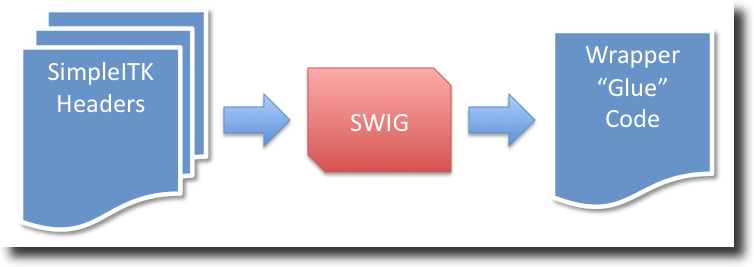
\includegraphics[width=.8\textwidth]{Images/WrappingProcess_shadow}
\end{center}
\begin{itemize}
  \item SimpleITK headers are constructed for wrapping
  \item SWIG is an open source package
  \begin{itemize}
    \item Parses C/C++ code, produces ``glue'' code
    \item Well supported, covers 10+ languages
  \end{itemize}
  \item Main languages: Python, Java, C\#
  \item Also supported: Tcl, Lua, R
\end{itemize}
\end{frame}

\begin{frame}[fragile]
\frametitle{Object Paradigm (Python)}
The paradigms translate to the wrapped languages (C++ $\rightarrow$ Python)
\lstcpp
\begin{lstlisting}
#include <SimpleITK.h>
using itk::simple;
...
// Create a smoothing filter
SmoothingRecursiveGaussianImageFilter gaussian;
// Set a parameter
gaussian.SetSigma ( 2.0 );
// "Execute" the Filter
Image blurredImage = gaussian.Execute ( image );
\end{lstlisting}
\lstpython
\begin{lstlisting}
from SimpleITK import *
# Create a smoothing filter
SmoothingRecursiveGaussianImageFilter gaussian
# Set a parameter
gaussian.SetSigma ( 2.0 );
# "Execute" the Filter
blurredImage = gaussian.Execute ( image );
\end{lstlisting}
\end{frame}

\begin{frame}[fragile]
\frametitle{Object Paradigm (Java)}
\lstjava
\begin{lstlisting}
import SimpleITK.*;
...

// Create a smoothing filter
SmoothingRecursiveGaussianImageFilter gaussian =
      new SmoothingRecursiveGaussianImageFilter();

// Set a parameter
gaussian.SetSigma ( 2.0 );

// "Execute" the Filter
Image blurredImage = gaussian.Execute ( image );
\end{lstlisting}
\end{frame}


\begin{frame}[fragile]
\frametitle{Object Paradigm (C\#)}
\lstjava
\begin{lstlisting}
using System;
using itk.simple;
...
// Create a smoothing filter
SmoothingRecursiveGaussianImageFilter gaussian =
      new SmoothingRecursiveGaussianImageFilter();

// Set a parameter
gaussian.SetSigma ( 2.0 );

// "Execute" the Filter
Image blurredImage = gaussian.Execute ( image );
\end{lstlisting}
\end{frame}


\begin{frame}{Note on the Tutorial}
\begin{itemize}
  \item Most examples will be Python
  \item Obvious translation to other languages
  \item C++ usage (generally) obvious
\end{itemize}
\end{frame}


\begin{frame}{Filters}
iPython examples
\end{frame}

\begin{frame}[fragile]
\frametitle{What just happened?}
\lstpython
\begin{lstlisting}
# Simple smoothing
smooth = SimpleITK.SmoothingRecursiveGaussian ( image, 2.0 )
SimpleITK.Show ( SimpleITK.Subtract ( image, smooth ) )
...
RuntimeError: Exception thrown in SimpleITK Subtract: ...
sitk::ERROR: Both images for SubtractImageFilter don't match type or dimension!
...
\end{lstlisting}

\begin{itemize}
  \item The output of SmoothingRecursiveGaussian is of type float
  \item The input image is signed short
  \item Most SimpleITK filters with 2 inputs require the same type
  \item Let's fix the problem
\end{itemize}

\end{frame}

\begin{frame}[fragile]
\frametitle{Introducing Cast}
\lstpython
\begin{lstlisting}
# Much better
smooth = SimpleITK.Cast ( smooth, image.GetPixelIDValue() )
print image.GetPixelIDTypeAsString()
print smooth.GetPixelIDTypeAsString()
SimpleITK.Show ( SimpleITK.Subtract ( image, smooth ) )
\end{lstlisting}
\end{frame}

%% Morphology
\subsection{Morphology}

\begin{frame}{Morphology}
\fontsize{36pt}{36pt}\selectfont
\center
\begin{center}
Morphology
\end{center}
\end{frame}

\begin{frame}[fragile]
\frametitle{Operators}

\begin{columns}[c]

\column{0.25\textwidth}
\begin{center}
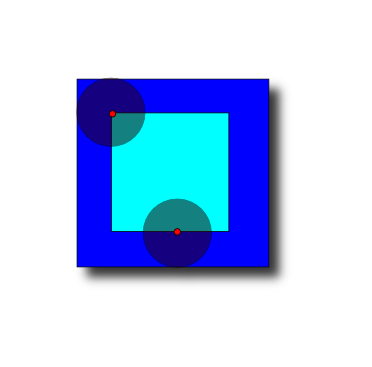
\includegraphics[width=1\textwidth]{Images/Erosion_shadow} \\
Erosion
\end{center}

\column{0.25\textwidth}
\begin{center}
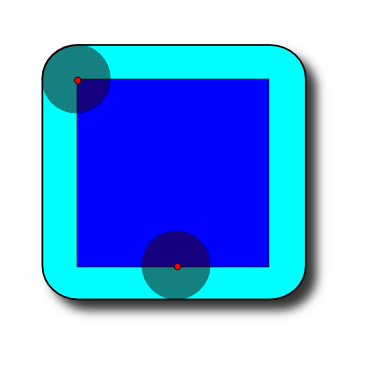
\includegraphics[width=1\textwidth]{Images/Dilation_shadow} \\
Dilation
\end{center}

\column{0.25\textwidth}
\begin{center}
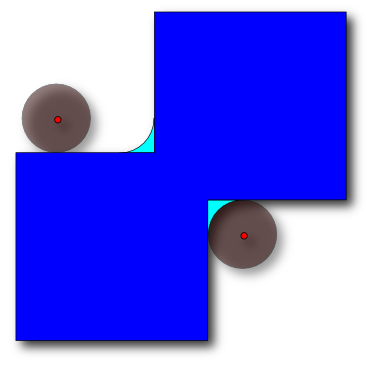
\includegraphics[width=1\textwidth]{Images/Closing_shadow} \\
Closing
\end{center}

\column{0.25\textwidth}
\begin{center}
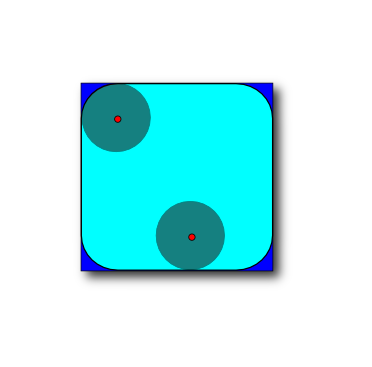
\includegraphics[width=1\textwidth]{Images/Opening_shadow} \\
Opening
\end{center}
\end{columns}
\vspace{12pt}
Images from \url{http://en.wikipedia.org/wiki/Mathematical_morphology}
\end{frame}

\begin{frame}{Morphology in Action}
\center
\begin{center}
Back to iPython
\end{center}
\end{frame}


\subsection{Label Maps}

%% Label maps
\begin{frame}{Label Maps}
\fontsize{36pt}{36pt}\selectfont
\center
\begin{center}
Label Maps
\end{center}
\end{frame}

%% Break
\begin{frame}{Break}
\fontsize{36pt}{36pt}\selectfont
\center
\begin{center}
Let's take a break
\end{center}
\end{frame}

